\subsection{Packet drop probability}

The probability that a packet needs to be retransmitted is

\begin{align*}
  p_{e,e2e} &= 1 - \prod_{k=1}^{r+1} (1 - p_{e,k})
\end{align*}

The probability that this exact packet will need to be retransmitted for the
$i^{th}$ time is independent of the $i-1$ number of times it was retransmitted
before. Hence, if $R$ is the number of maximum allowed transmission
attempts, the packet drop probability is

\begin{align*}
  p_{d,e2e} &= p_{d,e2e}^R = (1 - \prod_{k=1}^{r+1} (1 - p_{e,k}))^R
\end{align*}


% ------------------------------------------------------------------------------
\subsection{Packet loss ratio}

From the structure of the network:

\begin{align}
  \lambda_1 &= \lambda + \lambda_1 \cdot p_{e,e2e} - \lambda_1 \cdot p_{d,e2e} \nonumber \\
  \lambda_1 &= \dfrac{\lambda}{1 - p_{e,e2e} + p_{d,e2e}} \label{eq:07_lambda_1}
\end{align}

The number of error-free packets received at the mobile station (including it)
is
\begin{align*}
  \lambda_0 &= (1 - p_{e,e2e}) \lambda_1 - p_{d,e2e} \lambda_1 \\
  \dfrac{\lambda_0}{\lambda_1} &= 1 - p_{e,e2e} - p_{d,e2e} =
  \prod_{k=1}^{r+1} (1 - p_{e,k}) - (1 - \prod_{k=1}^{r+1} (1 - p_{e,k}))^R\\
\end{align*}

and from equation \ref{eq:07_lambda_1}

\begin{align*}
  \dfrac{\lambda_0}{\lambda} &= \dfrac{1 - p_{e,e2e} - p_{d,e2e}}{1 - p_{e,e2e} + p_{d,e2e}} =
  \dfrac{\prod\limits_{k=1}^{r+1} (1 - p_{e,k}) - (1 - \prod\limits_{k=1}^{r+1} (1 - p_{e,k}))^R}
        {\prod\limits_{k=1}^{r+1} (1 - p_{e,k}) + (1 - \prod\limits_{k=1}^{r+1} (1 - p_{e,k}))^R}
\end{align*}

Hence the packet loss ratio is

\begin{align*}
  \dfrac{\lambda - \lambda_0}{\lambda} = 1 - \dfrac{\prod\limits_{k=1}^{r+1} (1 - p_{e,k}) - (1 - \prod\limits_{k=1}^{r+1} (1 - p_{e,k}))^R}
        {\prod\limits_{k=1}^{r+1} (1 - p_{e,k}) + (1 - \prod\limits_{k=1}^{r+1} (1 - p_{e,k}))^R}
\end{align*}


% ------------------------------------------------------------------------------
\subsection{Stability region}

In order for this system to be stable the following should hold, with
$\lambda_i = \lambda_{r+1} = \lambda_1$:

\begin{align*}
  \dfrac{\lambda_i}{\mu_{AF}} &< 1 \\
  \dfrac{\lambda_{r+1}}{\mu_{MS}} &< 1
\end{align*}

Hence, due to $\mu_{MS} = \mu_{AF}$:

\begin{align*}
  \lambda &< \mu_{MS} (1 - p_{e,e2e} + p_{d,e2e}) \\
          &= \mu_{MS}\Big(\prod_{k=1}^{r+1} (1 - p_{e,k}) + (1 - \prod_{k=1}^{r+1} (1 - p_{e,k}))^R\Big)
\end{align*}

This stability region is larger than when there is no retransmission limit, as
was the case prior to this. This is reasonable, since, now, packets that need to
be retransmitted more times than this upper limit are not allowed to continue
their life-cycle in the system. The lower the value of $R$ is, the larger the
stability region is.


% ------------------------------------------------------------------------------
\subsection{Throughput}

From the packet loss ratio section:

\begin{align*}
  \lambda_0 &= \lambda\ \dfrac{1 - p_{e,e2e} - p_{d,e2e}}{1 - p_{e,e2e} + p_{d,e2e}} =
  \lambda\ \dfrac{\prod\limits_{k=1}^{r+1} (1 - p_{e,k}) - (1 - \prod\limits_{k=1}^{r+1} (1 - p_{e,k}))^R}
        {\prod\limits_{k=1}^{r+1} (1 - p_{e,k}) + (1 - \prod\limits_{k=1}^{r+1} (1 - p_{e,k}))^R} \\
\end{align*}


% ------------------------------------------------------------------------------
\subsection{Average end-to-end delay}

With similar reasoning to the first part of the theoretic analysis, the average
end-to-end delay is

\begin{align*}
  T &= \dfrac{1}{\mu_{MS}(1 - p_{e,e2e} + p_{d,e2e}) - \lambda} +
    \sum\limits_{i=1}^r \dfrac{1}{\mu_{AF}(1 - p_{e,e2e} + p_{d,e2e}) - \lambda} \\
    &= \dfrac{1}{\mu_{MS}\Big(\prod\limits_{k=1}^{r+1}(1-p_{e,k}) + (1 - \prod\limits_{k=1}^{r+1}(1-p_{e,k}))^R \Big) - \lambda} \\
    &+ \sum\limits_{i=1}^r \dfrac{1}{\mu_{AF}\Big(\prod\limits_{k=1}^{r+1}(1-p_{e,k}) + (1 - \prod\limits_{k=1}^{r+1}(1-p_{e,k}))^R \Big) - \lambda}
\end{align*}


Here we observe that the denominators in the expression of the average end-to-end
delay are increased due the introduction of the retransmission scheme. This
means that the delay is smaller in size, and, in fact, it is smaller for smaller
values of $R$.

% ------------------------------------------------------------------------------
\subsection{Numerical Evaluation}

Figure \ref{fig:07_packet_loss_ratio} shows the packet loss ratio as a function
of $R \in [3,8]$. The ratio of packets being dropped decreases as the number of
allowed retransmissions increases.

Figure \ref{fig:07_throughput_delay.tex} illustrates the relation between the
throughput and the average end-to-end delay for $\lambda = 0.9^5 + (1-0.9^5)^4$.
As the number of packets successfully delivered and processed by the mobile
station increases, so does the average time a packet has to wait until it is
successfully delivered and processed at the mobile station.

\begin{figure}[H]\centering
  % This file was created by matlab2tikz.
%
%The latest updates can be retrieved from
%  http://www.mathworks.com/matlabcentral/fileexchange/22022-matlab2tikz-matlab2tikz
%where you can also make suggestions and rate matlab2tikz.
%
\definecolor{mycolor1}{rgb}{0.00000,0.44700,0.74100}%
%
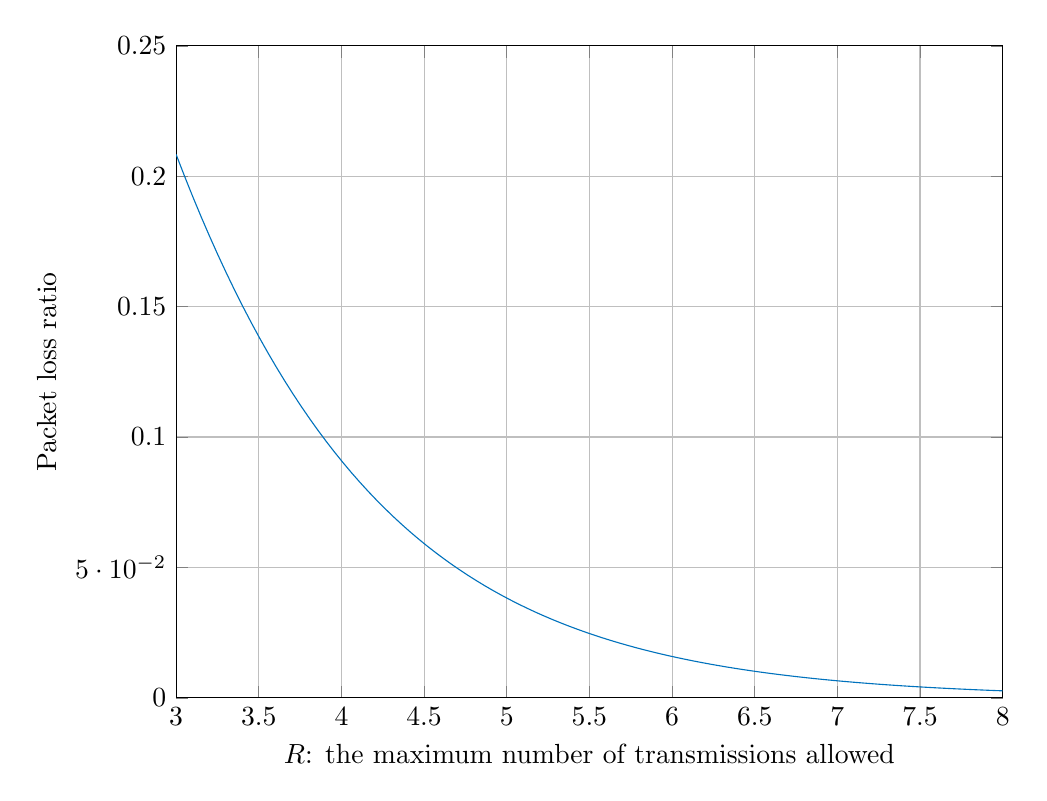
\begin{tikzpicture}

\begin{axis}[%
width=4.133in,
height=3.26in,
at={(0.693in,0.44in)},
scale only axis,
xmin=3,
xmax=8,
xmajorgrids,
xlabel={$R$: the maximum number of transmissions allowed},
ymin=0,
ymax=0.25,
ymajorgrids,
ylabel={Packet loss ratio},
axis background/.style={fill=white}
]
\addplot [color=mycolor1,solid,forget plot]
  table[row sep=crcr]{%
3	0.208367473337179\\
3.05050505050505	0.200099865257004\\
3.1010101010101	0.19212512196134\\
3.15151515151515	0.184435635223516\\
3.2020202020202	0.177023772155571\\
3.25252525252525	0.169881897006407\\
3.3030303030303	0.16300239124054\\
3.35353535353535	0.156377671947237\\
3.4040404040404	0.15000020863642\\
3.45454545454545	0.14386253848303\\
3.50505050505051	0.137957280085672\\
3.55555555555556	0.1322771458085\\
3.60606060606061	0.126814952777394\\
3.65656565656566	0.121563632602779\\
3.70707070707071	0.116516239901979\\
3.75757575757576	0.111665959693852\\
3.80808080808081	0.107006113737739\\
3.85858585858586	0.1025301658876\\
3.90909090909091	0.0982317265305632\\
3.95959595959596	0.0941045561771974\\
4.01010101010101	0.0901425682685546\\
4.06060606060606	0.0863398312626219\\
4.11111111111111	0.0826905700601598\\
4.16161616161616	0.0791891668272006\\
4.21212121212121	0.0758301612686363\\
4.26262626262626	0.0726082504044635\\
4.31313131313131	0.0695182878973829\\
4.36363636363636	0.0665552829775643\\
4.41414141414141	0.0637143990075706\\
4.46464646464646	0.0609909517276483\\
4.51515151515152	0.0583804072188784\\
4.56565656565657	0.0558783796190719\\
4.61616161616162	0.0534806286237394\\
4.66666666666667	0.051183056802049\\
4.71717171717172	0.048981706755352\\
4.76767676767677	0.0468727581436387\\
4.81818181818182	0.0448525246031876\\
4.86868686868687	0.0429174505766724\\
4.91919191919192	0.0410641080751224\\
4.96969696969697	0.0392891933893533\\
5.02020202020202	0.0375895237668373\\
5.07070707070707	0.0359620340684281\\
5.12121212121212	0.0344037734179063\\
5.17171717171717	0.0329119018559699\\
5.22222222222222	0.0314836870090358\\
5.27272727272727	0.0301165007820726\\
5.32323232323232	0.0288078160835938\\
5.37373737373737	0.0275552035899752\\
5.42424242424242	0.026356328555335\\
5.47474747474747	0.025208947672387\\
5.52525252525253	0.0241109059889126\\
5.57575757575758	0.0230601338837962\\
5.62626262626263	0.0220546441059367\\
5.67676767676768	0.021092528878759\\
5.72727272727273	0.0201719570725382\\
5.77777777777778	0.0192911714462538\\
5.82828282828283	0.0184484859602824\\
5.87878787878788	0.017642283160835\\
5.92929292929293	0.0168710116367091\\
5.97979797979798	0.0161331835486054\\
6.03030303030303	0.0154273722309968\\
6.08080808080808	0.0147522098662782\\
6.13131313131313	0.0141063852307189\\
6.18181818181818	0.0134886415115442\\
6.23232323232323	0.0128977741943084\\
6.28282828282828	0.012332629019582\\
6.33333333333333	0.0117921000078363\\
6.38383838383838	0.011275127551323\\
6.43434343434343	0.0107806965716408\\
6.48484848484848	0.0103078347416112\\
6.53535353535354	0.00985561077002817\\
6.58585858585859	0.00942313274779083\\
6.63636363636364	0.00900954655389008\\
6.68686868686869	0.00861403431970398\\
6.73737373737374	0.00823581295001408\\
6.78787878787879	0.00787413269916759\\
6.83838383838384	0.00752827580078608\\
6.88888888888889	0.0071975551494361\\
6.93939393939394	0.00688131303267492\\
6.98989898989899	0.00657891991189996\\
7.04040404040404	0.00628977325044699\\
7.09090909090909	0.00601329638740078\\
7.14141414141414	0.00574893745559868\\
7.19191919191919	0.00549616834234612\\
7.24242424242424	0.00525448369137593\\
7.29292929292929	0.00502339994461887\\
7.34343434343434	0.00480245442239025\\
7.39393939393939	0.00459120444061389\\
7.44444444444444	0.00438922646375861\\
7.49494949494949	0.00419611529217168\\
7.54545454545455	0.00401148328255518\\
7.5959595959596	0.00383495960034397\\
7.64646464646465	0.00366618950278963\\
7.6969696969697	0.00350483365159049\\
7.74747474747475	0.00335056745393891\\
7.7979797979798	0.00320308043089013\\
7.84848484848485	0.00306207561200533\\
7.8989898989899	0.00292726895523066\\
7.94949494949495	0.00279838879103522\\
8	0.00267517528984562\\
};
\end{axis}
\end{tikzpicture}%

  \caption{The packet loss ratio for $R \in [3,8]$, $\mu_{AF} = \mu_{MS} = 2$,
    $p_{e,i} = 0.1$, $r=4$ and $\lambda = 0.5 \lambda_{max}(r)$.}
  \label{fig:07_packet_loss_ratio}
\end{figure}

\begin{figure}\centering
  % This file was created by matlab2tikz.
%
%The latest updates can be retrieved from
%  http://www.mathworks.com/matlabcentral/fileexchange/22022-matlab2tikz-matlab2tikz
%where you can also make suggestions and rate matlab2tikz.
%
\definecolor{mycolor1}{rgb}{0.00000,0.44700,0.74100}%
%
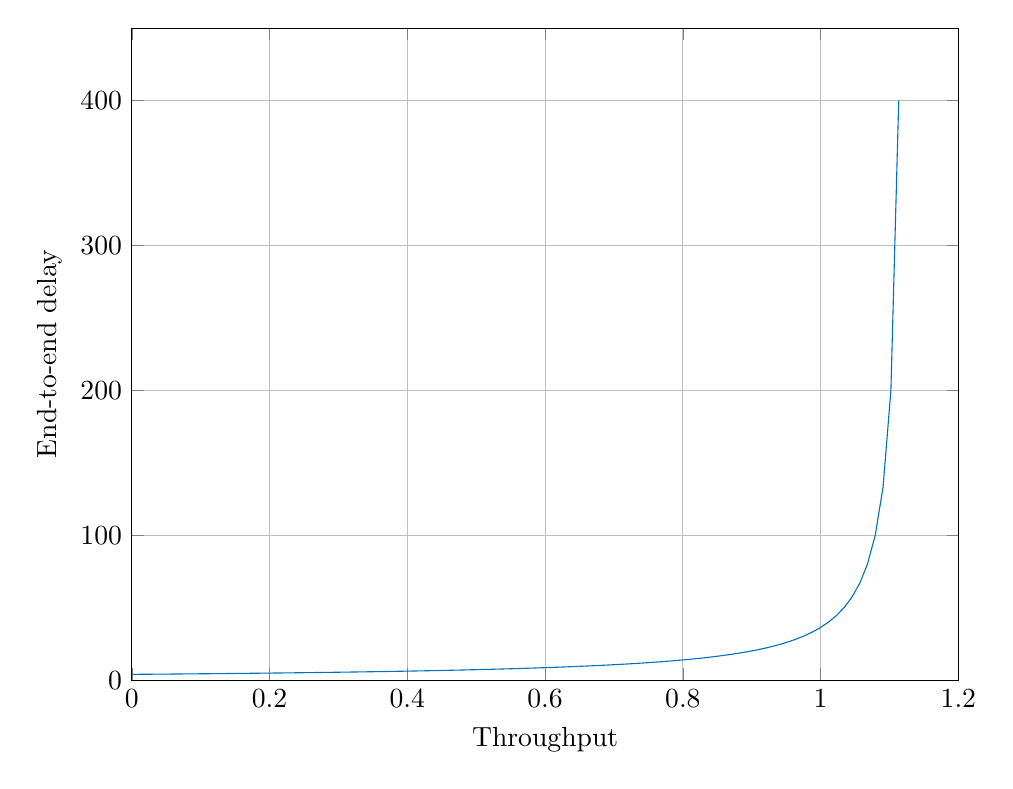
\begin{tikzpicture}

\begin{axis}[%
width=4.133in,
height=3.26in,
at={(0.693in,0.44in)},
scale only axis,
unbounded coords=jump,
xmin=0,
xmax=1.2,
xmajorgrids,
xlabel={Throughput},
ymin=0,
ymax=450,
ymajorgrids,
ylabel={End-to-end delay},
axis background/.style={fill=white}
]
\addplot [color=mycolor1,solid,forget plot]
  table[row sep=crcr]{%
0	4.04130036449744\\
0.0113609542058187	4.08253812331885\\
0.0227219084116374	4.12462614520873\\
0.0340828626174562	4.16759100088799\\
0.0454438168232749	4.2114603798447\\
0.0568047710290936	4.25626314984305\\
0.0681657252349123	4.30202942027147\\
0.0795266794407311	4.34879060962225\\
0.0908876336465498	4.3965795174203\\
0.102248587852369	4.44543040094719\\
0.113609542058187	4.49537905713761\\
0.124970496264006	4.54646291005962\\
0.136331450469825	4.59872110442813\\
0.147692404675643	4.65219460564241\\
0.159053358881462	4.70692630688526\\
0.170414313087281	4.76296114387199\\
0.1817752672931	4.82034621789454\\
0.193136221498918	4.87913092786887\\
0.204497175704737	4.93936711216354\\
0.215858129910556	5.00110920106559\\
0.227219084116374	5.06441438082591\\
0.238580038322193	5.12934277032368\\
0.249940992528012	5.19595761149671\\
0.261301946733831	5.26432547480588\\
0.272662900939649	5.33451648113663\\
0.284023855145468	5.40660454169253\\
0.295384809351287	5.48066761760612\\
0.306745763557106	5.55678800118399\\
0.318106717762924	5.63505262091897\\
0.329467671968743	5.71555337264639\\
0.340828626174562	5.79838747949633\\
0.35218958038038	5.88365788360657\\
0.363550534586199	5.97147367291413\\
0.374911488792018	6.06195054674617\\
0.386272442997837	6.15521132438841\\
0.397633397203655	6.25138650133198\\
0.408994351409474	6.35061485849598\\
0.420355305615293	6.45304413040721\\
0.431716259821112	6.55883173910241\\
0.44307721402693	6.66814560142078\\
0.454438168232749	6.78116501839402\\
0.465799122438568	6.89808165664219\\
0.477160076644387	7.01910063307451\\
0.488521030850205	7.14444171580798\\
0.499881985056024	7.2743406560954\\
0.511242939261843	7.40905066824531\\
0.522603893467661	7.54884407708013\\
0.53396484767348	7.69401415548552\\
0.545325801879299	7.8448771781421\\
0.556686756085117	8.00177472170494\\
0.568047710290936	8.16507624663769\\
0.579408664496755	8.33518200177598\\
0.590769618702574	8.51252629968611\\
0.602130572908392	8.6975812192445\\
0.613491527114211	8.89086080189438\\
0.62485248132003	9.09292582011925\\
0.636213435525849	9.30438921128481\\
0.647574389731667	9.52592228774398\\
0.658935343937486	9.75826185573773\\
0.670296298143305	10.0022184021312\\
0.681657252349123	10.2586855406474\\
0.693018206554942	10.5286509496118\\
0.704379160760761	10.8132090833851\\
0.71574011496658	11.113576002368\\
0.727101069172398	11.4311067452928\\
0.738462023378217	11.7673157672131\\
0.749822977584036	12.1239010934923\\
0.761183931789855	12.502773002664\\
0.772544885995673	12.9060882608144\\
0.783905840201492	13.3362912028416\\
0.795266794407311	13.7961633132844\\
0.806627748613129	14.288883431616\\
0.817988702818948	14.8181013364906\\
0.829349657024767	15.388028310971\\
0.840710611230586	16.0035494434099\\
0.852071565436404	16.670364003552\\
0.863432519642223	17.395162438489\\
0.874793473848042	18.1858516402385\\
0.886154428053861	19.051844575488\\
0.897515382259679	20.0044368042623\\
0.908876336465498	21.0573018992235\\
0.920237290671317	22.2271520047359\\
0.931598244877135	23.5346315344263\\
0.942959199082954	25.0055460053279\\
0.954320153288773	26.6725824056832\\
0.965681107494592	28.5777668632319\\
0.97704206170041	30.7760566219421\\
0.988403015906229	33.3407280071039\\
0.999763970112048	36.371703280477\\
1.01112492431787	40.0088736085247\\
1.02248587852369	44.4543040094719\\
1.0338468327295	50.0110920106558\\
1.04520778693532	57.1555337264639\\
1.05656874114114	66.6814560142079\\
1.06792969534696	80.0177472170496\\
1.07929064955278	100.022184021312\\
1.0906516037586	133.362912028416\\
1.10201255796442	200.044368042624\\
1.11337351217023	400.088736085245\\
1.12473446637605	inf\\
};
\end{axis}
\end{tikzpicture}%

  \caption{The relation between the throughput and the average end-to-end delay
    for $R=4$, $\mu_{AF} = \mu_{MS} = 2$, $p_{e,i} = 0.1$, $r=4$ and
    $\lambda < \lambda_{max}(r)$.}
  \label{fig:07_throughput_delay.tex}
\end{figure}
